\documentclass{article}

\usepackage{amsmath,amssymb}
\usepackage{graphicx}
\usepackage[utf8]{inputenc}

% Notation
% Mathematical functions
\newcommand{\isone}[1]{{\boldsymbol{1}\left( #1 \right)}}
\renewcommand{\Pr}[1]{{\mathbb{P}\left(#1\right) }}
\newcommand{\f}[1]{{f\left(#1\right) }}
\newcommand{\Prcond}[2]{{\mbox{Pr}\left(#1\vphantom{#2}\;\right|\left.\vphantom{#1}#2\right)}}
\newcommand{\fcond}[2]{{f\left(#1|#2\right) }}
\newcommand{\Expected}[1]{{\mathbb{E}\left\{#1\right\}}}
\newcommand{\ExpectedCond}[2]{{\mathbb{E}\left\{#1\vphantom{#2}\;\right|\left.\vphantom{#1}#2\right\}}}

\newcommand{\Likelihood}[2]{\text{L}\left(#1 \left|\vphantom{#1}#2\right.\right)}
\newcommand{\sufstats}[1]{s\left(#1\right)}
\renewcommand{\exp}[1]{\mbox{exp}\left\{#1\right\}}
\newcommand{\transpose}[1]{{#1}^\mathbf{t}}

% Objects
\newcommand{\params}{\theta}
\newcommand{\Params}{\Theta}
\newcommand{\Graph}{\mathbf{G}}
\newcommand{\graph}{\mathbf{g}}
\newcommand{\GRAPH}{\mathcal{G}}
\newcommand{\Adjmat}{Y}
\newcommand{\adjmat}{y}
\newcommand{\ADJMAT}{\mathcal{Y}}

\newcommand{\INDEPVAR}{\mathcal{X}}
\newcommand{\Indepvar}{X}
\newcommand{\indepvar}{x}

\newcommand{\normconst}{\kappa\left(\params, \Indepvar\right)}

% \graphicspath{{./fig/}}


%% NEED THIS FOR CANCY TEX
\usepackage{pstricks}

% Colors
\definecolor{USCCardinal}{HTML}{990000} % 153 0 0 in RGB
\definecolor{USCGold}{HTML}{FFCC00}
\definecolor{USCGray}{HTML}{CCCCCC}

% To use the function \sout
\usepackage{ulem}
\usepackage{tabularx, booktabs}

% \bibliography{bibliography.bib}

\title{Exponential Random Graph models for Little Networks}
\author{George G. Vega Yon \and Kayla de la Haye}
\date{January 2019}

\begin{document}

\maketitle

To be submitted at https://arxiv.org/help/submit

\section{Introduction}

Exponential-Family Graph Models (ERGMs), are certainly one of the most popular tools used by social scientists interested on understanding social networks.

\begin{equation}
\label{eq:ergm}
  \Prcond{\Adjmat = \adjmat}{\params, \Indepvar} = \frac{%
  	\exp{\transpose{\params}\sufstats{\adjmat, \Indepvar}}%	
  }{
  	\kappa\left(\params, \Indepvar\right)
  },\quad\forall \adjmat\in\ADJMAT
\end{equation}

Where $\normconst{} = \sum_{\adjmat\in\ADJMAT}\exp{\transpose{\theta}\sufstats{\adjmat, \Indepvar}}$ is the normalizing constant.

\def\fig1width{.45\linewidth}
\begin{figure}
\centering
\begin{tabular}{m{.2\linewidth}<\centering m{.4\linewidth}<\raggedright}
\toprule Representation & Description  \\ \midrule

\includegraphics[width=\fig1width]{terms/mutual.pdf} & Mutual Ties (Reciprocity)\linebreak[4]$\sum_{i\neq j}y_{ij}y_{ji}$  \\
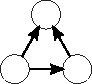
\includegraphics[width=\fig1width]{terms/ttriad.pdf} & Transitive Triad (Balance)\linebreak[4]$\sum_{i\neq j\neq k}y_{ij}y_{jk}y_{ik}$  \\

\includegraphics[width=\fig1width]{terms/homophily.pdf} & Homophily\linebreak[4]$\sum_{i\neq j}y_{ij}\mathbf{1}\left(x_i=x_j\right)$ \\
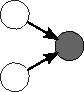
\includegraphics[width=\fig1width]{terms/nodeicov.pdf} & Covariate Effect for Incoming Ties\linebreak[4]$\sum_{i\neq j}y_{ij}x_j$ \\
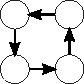
\includegraphics[width=\fig1width]{terms/fourcycle.pdf} & Four Cycle\linebreak[4]$\sum_{i\neq j \neq k \neq l}y_{ij}y_{jk}y_{kl}y_{li}$  \\
\bottomrule
\end{tabular}
\caption{\label{fig:ergm-structs}Besides of the common edge count statistic (number of ties in a graph), ERGMs allow measuring other more complex structures that can be captured as sufficient statistics. }
\end{figure}

\section{Estimation of {\it ERGMitos}}

What is small? It depends, in the case of simple networks--undirected graphs--the support has has $2^{n(n-1)/2}$ networks, which means that for a graph of size 7 there are 2,097,152 possible networks to be considered in the model. From the practical point of view, this actually is more simple as the exhaustive enumeration of graphs has to be done only once, in particular, let $\mathcal{W}(m)$ be the powerset of vector statistics associated with model $m$, $q(w)\equiv |\{y\in\mathcal{Y}: s(y,x) = w\}|$, then \eqref{eq:ergm} can be expressed as:

\section{Simulation study}

We conducted a simulation study to explore the properties of MLE for small networks. To generate each sample of teams:

1. Draw the **population parameters** from a piece-wise Uniform with values in $[-4, -.1]\cup[.1, 4]$

2. We will draw groups of sizes 3 to 5. The number of networks per group size are drawn from a Poisson distribution with parameter 10 (hence, an expected size of 30 networks per sample).

3. Use the drawn parameters and group sizes to generate random graphs using an ERGM data generating process.

We simulated 100,000 samples, each one composed of an average of 30 networks.

\section{References}

\appendix

\section{Gradient function}

\begin{equation}
\nabla l(\theta) = \transpose{\stats{\Mat{x}}} - \frac{\transpose{\Mat{Q}}\left(\transpose{\Mat{W}} \circ \exp{\Mat{Q} \theta}\right)}{\kappa}
\end{equation}

\end{document}
